\section*{Exercice 132 -- Statique}
\setcounter{exo}{0}
%POLE JC

Un lève-personne est un dispositif médical utilisé dans les maisons
de retraites ou les hôpitaux. C’est une aide technique mécanisée qui
sert à effectuer des transferts de personnes qui n’ont pas la
capacité de se déplacer en autonomie.
Le transfert le plus courant est celui qui consiste à transporter le
patient du lit vers le fauteuil et inversement.
Le système étudié fonctionne grâce à l’énergie électrique fournie
par des batteries rechargeables.
Un modèle du mécanisme est représenté ci-dessous. Il est
constitué :
\begin{itemize}
\item d’un support (0) de repère associé $\rep{0}= \repere{O}{x_0}{y_0}{z_0}$;
\item d’un ensemble (1) (bras + malade), de repère associé $\rep{1}= \repere{O}{x_1}{y_0}{z_0}$; , de masse maximale $m$ et de centre de gravité $G$ tel que $\vect{OG} = a \vect{x_0} + y(t) \vect{y_0}$.
\end{itemize}

Les sollicitations proviennent :
\begin{itemize}
\item d’un vérin d’élévation électrique assurant le déplacement vertical
de l’ensemble (1). Sa poussée est une force de droite d’action (AB)
et de résultante $F_v \vect{y_0}$ avec $\vect{OA} = -b \vect{x_0} + c\vect{y_0}$;
\item d’un ressort de compression placé entre (0) et (1), permettant de compenser une partie du poids du malade et soulager ainsi le vérin.
Il exerce entre (0) et (1) une force de droite d’action $\axe{O}{y_0}$, de
résultante $-k(y - y0) \vect{y_0}$ , avec $k$ sa raideur en N/m et $y_0$ une
constante dépendant de la longueur à vide du ressort ;
\item du poids de l’ensemble, force de résultante $-mg \vect{y_0}$ passant par $G$;
\item la liaison glissière (parfaite) exerce une action qu'on peut exprimer en $O$.
\end{itemize}


\begin{center}
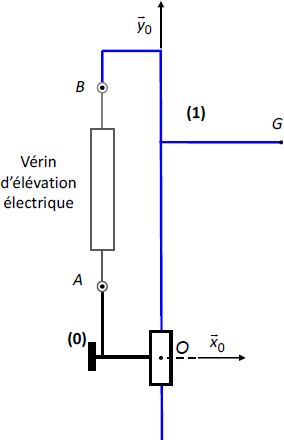
\includegraphics[width=.6\linewidth]{095_02}
\end{center}


\begin{obj}
Afin de dimensionner les constituants qui les réalisent, déterminer les actions transmises par le
vérin et la liaison entre (1) et (0).
\end{obj}

\subparagraph{}\textit{Positionner sur le schéma, à l’aide de vecteurs, les résultantes des actions mécaniques du vérin, du ressort et de la
pesanteur.}
\ifprof
\begin{corrige}
\end{corrrige}
\else
\fi


\subparagraph{}\textit{Réaliser le graphe de structure.}
\ifprof
\begin{corrige}
\end{corrrige}
\else
\fi


\subparagraph{}\textit{Isoler 1 et déterminer, lorsque le mécanisme est à l’équilibre, les 6 équations issues du PFS exprimé en $O$.}
\ifprof
\begin{corrige}
\end{corrrige}
\else
\fi


\subparagraph{}\textit{En déduire l’expression, de l’effort de poussée du vérin $F_v$ en fonction de $m$, $g$, $k$, $y$ et $y_0$.}
\ifprof
\begin{corrige}
\end{corrrige}
\else
\fi


\subparagraph{}\textit{Exprimer le torseur des actions mécaniques transmises par la liaison entre 1 et 0 en fonction de $m$,$g$, $a$, $b$, $k$, $y$ et $y_0$.}
\ifprof
\begin{corrige}
\end{corrrige}
\else
\fi

